The {\sundials} suite (or individual solvers) are distributed as
compressed archives (\id{.tar.gz}). The name of the distribution
archive is of the form {\em solver}\id{-x.y.z.tar.gz}, where {\em
solver} is one of: \id{sundials}, \id{cvode}, \id{cvodes}, \id{ida},
\id{idas}, or \id{kinsol}, and \id{x.y.z} represents the version number
(of the {\sundials} suite or of the individual solver).
%%
To begin the installation, first uncompress and expand the sources, by issuing
\begin{verbatim}
   % tar xzf solver-x.y.z.tar.gz
\end{verbatim}
This will extract source files under a directory {\em solver}\id{-x.y.z}.

Starting with version \id{2.8.0} of {\sundials}, CMake is the only supported method
of installation.
Before providing detailed explanations on the installation procedure, we begin with a few common observations:
%%
\begin{itemize}

\item In the remainder of this chapter, we make the following distinctions:
  \begin{description}
  \item[{\em srcdir}] 
    is the directory {\em solver}\id{-x.y.z} created above; i.e., the 
    directory containing the {\sundials} sources.
  \item[{\em builddir}]
    is the (temporary) directory under which {\sundials} is built.
  \item[{\em instdir}]
    is the directory under which the {\sundials} exported header files
    and libraries will be installed. Typically, header files are exported under a directory
    {\em instdir}\id{/include} while libraries are installed under {\em instdir}\id{/lib},
    with {\em instdir} specified at configuration time.
  \end{description}

\item For {\sundials} CMake-based installation, in-source builds are prohibited; in other words, the
  build directory {\em builddir} can {\bf not} be the same as {\em srcdir}
  and such an attempt will lead to an error. This
  prevents ``polluting'' the source tree and allows efficient builds
  for different configurations and/or options.

\item {\warn}The installation directory {\em instdir} can {\bf not} be the same as
  the source directory {\em srcdir}.

\item By default, only the libraries and header files are exported to the installation
  directory {\em instdir}.  If enabled by the user (with the
  appropriate toggle for CMake), the
  examples distributed with {\sundials} will be built together with
  the solver libraries but the installation step will result in
  exporting (by default in a subdirectory of the installation
  directory) the example sources and sample outputs together with
  automatically generated configuration files that reference the {\em
  installed} {\sundials} headers and libraries.  As such, these
  configuration files for the {\sundials} examples can be used as
  "templates" for your own problems. CMake installs \id{CMakeLists.txt} files and also
  (as an option available only under Unix/Linux) makefiles. Note this
  installation approach also allows the option of building the
  {\sundials} examples without having to install them.  (This can be
  used as a sanity check for the freshly built libraries.)

\item Even if generation of shared libraries is enabled, only static libraries
  are created for the FCMIX modules.  (Because of the use of fixed names for
  the Fortran user-provided subroutines, FCMIX shared libraries would result in
  "undefined symbol" errors at link time.)

\end{itemize}


%%===============================================================================
\section{CMake-based installation}\label{s:cmake_inst}
%%===============================================================================

CMake-based installation provides a platform-independent build system. CMake can generate
Unix/Linux Makefiles, as well as KDevelop, Visual Studio, and 
(Apple) XCode project files from the same configuration file.
In addition, CMake also provides a GUI front end and which allows an interactive build and
installation process.

The {\sundials} build process requires CMake version \id{2.8.1} or
higher and a working compiler.  On Unix-like operating systems, it
also requires Make (and \id{curses}, including its development libraries,
for the GUI front end to CMake, \id{ccmake}), while on Windows it
requires Visual Studio.  While many Linux distributions offer CMake,
the version included is probably out of date.  Many new CMake
features have been added recently, and you should download the latest
version from {\tt http://www.cmake.org}.  Build instructions for CMake
(only necessary for Unix-like systems) can be found on the CMake website.
Once CMake is installed, Linux/Unix users will be able to use \id{ccmake},
while Windows users will be able to use \id{CMakeSetup}.

As previously noted, when using CMake to configure, build and install {\sundials}, it is always
required to use a separate build directory. While in-source builds are possible, they are
explicitly prohibited by the {\sundials} CMake scripts (one of the reasons being that, unlike
autotools, CMake does not provide a \id{make distclean} procedure and it is therefore
difficult to clean-up the source tree after an in-source build).

\subsection{Configuring, building, and installing on Unix-like systems}

The default CMake configuration will build all included solvers and associated examples
and will only build static libraries. The {\em instdir} defaults to /usr/local and can be changed
by setting the \id{CMAKE\_INSTALL\_PREFIX} variable.
Support for FORTRAN, shared libraries and all other options are disabled.

CMake can be used from the command line with the \id{cmake} command, or from a Curses based GUI
by using the \id{ccmake} command. Examples for using both methods will be presented.
For the examples shown it is assumed that there is a top level {\sundials} directory
with appropriate source, build and install directories:

\begin{verbatim}
   % mkdir (...)sundials/instdir
   % mkdir (...)sundials/builddir
   % cd (...)sundials/builddir
\end{verbatim}

%%
%% Building with the GUI configuration
%%
\subsubsection*{Building with the GUI}

Using CMake with the GUI follows this general process:  
\begin{itemize}
\item Select and modify values, run configure (\id{c} key)
\item New values are denoted with an asterisk
\item To set a variable, move the cursor to the variable and press enter
  \begin{itemize}
  \item If it is a boolean (ON/OFF) it will flip the value
  \item If it is string or file, it will allow editing of the string
  \item For file and directories, the \id{<tab>} key can be used to complete 
  \end{itemize}
\item Repeat until all values are set as desired and the generate option is available (\id{g} key)
\item Some variables (advanced variables) are not visible right away
\item To see advanced variables, toggle to advanced mode (\id{t} key)
\item To search for a variable press \id{/} key, and to repeat the search, press the
\id{n} key
\end{itemize}

To build the default configuration using the GUI, from the {\em builddir} enter
the ccmake command and point to the {\em sourcedir}:

\begin{verbatim}
    % ccmake ../sourcedir
\end{verbatim}

The default configuration screen is shown in Figure
\ref{f:ccmakedefault}. 
\begin{figure}
{\centerline{\psfig{figure=ccmakedefault.eps,width=\textwidth}}}
%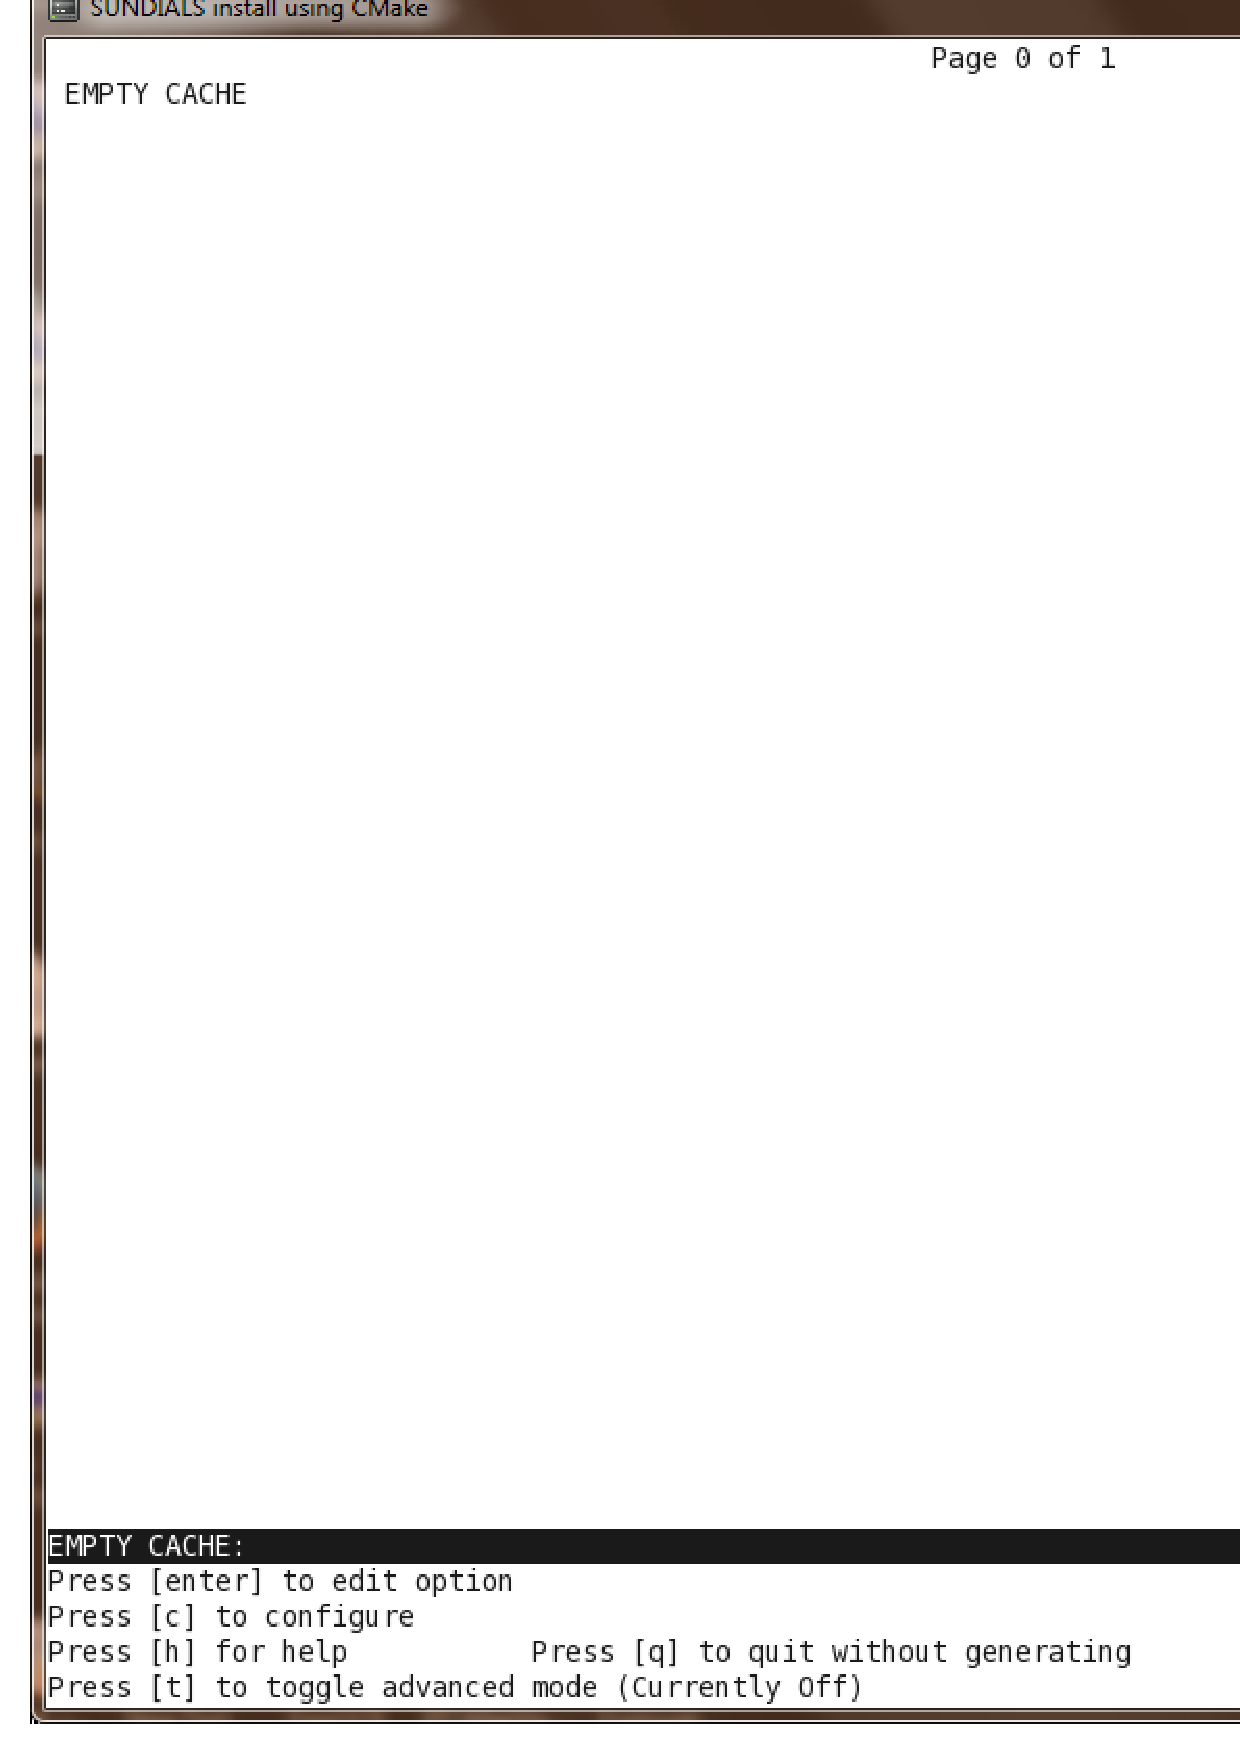
\includegraphics[width=\textwidth]{ccmakeempty.png}
\caption [Initial {\em ccmake} configuration screen]
{Default configuration screen. Note: Initial screen is empty.
Press 'c' to get this initial default configuration.}
\label{f:ccmakedefault}
\end{figure}

The default {\em instdir} for both {\sundials} and corresponding examples
can be changed by setting the \id{CMAKE\_INSTALL\_PREFIX} and
the \id{EXAMPLES\_INSTALL\_PATH} as shown in figure
\ref{f:ccmakeprefix}. 
\begin{figure}
{\centerline{\psfig{figure=ccmakeprefix.eps,width=\textwidth}}}
\caption [Changing the {\em instdir}]
{Changing the {\em instdir} for {\sundials} and
corresponding {\id examples} }
\label{f:ccmakeprefix}
\end{figure}

Pressing the (\id{g} key) will generate makefiles including all dependencies
and all rules to build {\sundials} on this system. 
Back at the command prompt, you can now type:

\begin{verbatim}
  % make
\end{verbatim}

To install {\sundials} in the installation directory specified in the configuration, simply run:

\begin{verbatim}
  % make install
\end{verbatim}

The distribution of {\sundials} includes several examples corresponding to the solvers to be
installed. Also included in the source bundle is a {\em testRunner} configured by CMake
to test these included examples:

\begin{verbatim}
  % make test
\end{verbatim}

The output of {\em testRunner} should look similar to figure
\ref{f:cmaketest}. 
\begin{figure}
%{\centerline{\psfig{figure=cmaketest.eps,width=\textwidth}}}
%\caption [Running {\em testRunner}]
%{Invoking {\em testRunner} with {\id make test} to execute all configured
%{\id examples} }
\label{f:cmaketest}
\end{figure}

%%
%% Building from the command line
%%
\subsubsection*{Building from the command line}

Using CMake from the command line is simply a matter of specifying CMake variable settings
with the {\id cmake} command.  The following will build the same configuration as shown above:  

\begin{verbatim}
   % cmake -DCMAKE_INSTALL_PREFIX=/usr/casc/sundials/installdir \
   > -DEXAMPLES_INSTALL_PATH=/usr/casc/sundials/installdir \
   > ../sourcedir
   % make
   % make test
\end{verbatim}


\subsection{Configuration options}

A complete list of all available options for a CMake-based {\sundials}
configuration is provide below. Note that the default values shown are for 
a typical configuration on a Linux system and are provided as illustration only.
Some of them will be different on different systems.

\begin{description}
\item[\id{BUILD\_CVODE}] - 
  Build the CVODE library 
  \\
  Default: ON
\item[\id{BUILD\_CVODES}] - 
  Build the CVODES library 
  \\
  Default: ON
\item[\id{BUILD\_IDA}] - 
   Build the IDA library 
  \\
   Default: ON
\item[\id{BUILD\_IDAS}] - 
  Build the IDAS library 
  \\
  Default: ON
\item[\id{BUILD\_KINSOL}] - 
  Build the KINSOL library 
  \\
  Default: ON
\item[\id{BUILD\_SHARED\_LIBS}] - 
  Build shared libraries
  \\
  Default: OFF 
\item[\id{BUILD\_STATIC\_LIBS}] - 
  Build static libraries
  \\
  Default: ON 
\item[\id{CMAKE\_BUILD\_TYPE}] -  
  Choose the type of build, options are: 
  None (CMAKE\_C\_FLAGS used) Debug Release RelWithDebInfo MinSizeRel
  \\
  Default:
\item[\id{CMAKE\_C\_COMPILER}] - 
  C compiler
  \\
  Default: /usr/bin/gcc 
\item[\id{CMAKE\_C\_FLAGS}] -  
  Flags for C compiler
  \\
  Default:
\item[\id{CMAKE\_C\_FLAGS\_DEBUG}] -      
  Flags used by the compiler during debug builds
  \\
  Default: -g 
\item[\id{CMAKE\_C\_FLAGS\_MINSIZEREL}] -  
  Flags used by the compiler during release minsize builds
  \\
  Default: -Os -DNDEBUG 
\item[\id{CMAKE\_C\_FLAGS\_RELEASE}] -    
  Flags used by the compiler during release builds
  \\
  Default: -O3 -DNDEBUG 
\item[\id{CMAKE\_BACKWARDS\_COMPATIBILITY}] - 
  For backwards compatibility, what version of CMake commands and
  syntax should this version of CMake allow.
  \\
  Default: 2.4
\item[\id{CMAKE\_Fortran\_COMPILER}] - 
  Fortran compiler
  \\
  Default: /usr/bin/g77
  \\
  Note: Fortran support (and all related options) are triggered only if
  either Fortran-C support is enabled (\id{FCMIX\_ENABLE} is ON) or
  Blas/Lapack support is enabled (\id{LAPACK\_ENABLE} is ON).
\item[\id{CMAKE\_Fortran\_FLAGS}] - 
  Flags for Fortran compiler
  \\
  Default:
\item[\id{CMAKE\_Fortran\_FLAGS\_DEBUG}] - 
  Flags used by the compiler during debug builds
  \\
  Default:
\item[\id{CMAKE\_Fortran\_FLAGS\_MINSIZEREL}] - 
  Flags used by the compiler during release minsize builds
  \\
  Default:
\item[\id{CMAKE\_Fortran\_FLAGS\_RELEASE}] - 
  Flags used by the compiler during release builds
  \\
  Default:
\item[\id{CMAKE\_INSTALL\_PREFIX}] -   
  Install path prefix, prepended onto install directories
  \\
  Default: /usr/local 
  \\
  Note: The user must have write access to the location specified through
  this option. Exported {\sundials} header files and libraries will be 
  installed under subdirectories \id{include} and \id{lib} of 
  \id{CMAKE\_INSTALL\_PREFIX}, respectively.
\item[\id{EXAMPLES\_ENABLE}] -   
  Build the {\sundials} examples
  \\
  Default: OFF
  \\
  Note: setting this option to ON will trigger additional options
  related to how and where example programs will be installed.
\item[\id{EXAMPLES\_GENERATE\_MAKEFILES}] - 
  Create Makefiles for building the examples
  \\
  Default: ON
  \\
  Note: This option is triggered only if enabling the building and installing of
  the example programs (i.e., both \id{EXAMPLES\_ENABLE} and \id{EXAMPLEs\_INSTALL}
  are set to ON) and if configuration is done on a Unix-like system. If enabled,
  makefiles for the compilation of the example programs (using the installed
  {\sundials} libraries) will be automatically generated and exported to the directory
  specified by \id{EXAMPLES\_INSTALL\_PATH}.
\item[\id{EXAMPLES\_INSTALL}] - 
  Install example files
  \\
  Default: ON
  \\
  Note: This option is triggered only if building example programs
  is enabled (\id{EXAMPLES\_ENABLE} ON). If the user requires
  installation of example programs then the sources and sample output files
  for all {\sundials} modules that are currently enabled will be exported to
  the directory specified by \id{EXAMPLES\_INSTALL\_PATH}. A CMake configuration
  script will also be automatically generated and exported to the same directory.
  Additionally, if the configuration is done under a Unix-like system, an additional
  option (\id{EXAMPLES\_GENERATE\_MAKEFILES}) will be triggered.
\item[\id{EXAMPLES\_INSTALL\_PATH}] - 
  Output directory for installing example files
  \\
  Default: /usr/local/examples
  \\
  Note: The actual default value for this option will an \id{examples}
  subdirectory created under \id{CMAKE\_INSTALL\_PREFIX}.
\item[\id{EXAMPLES\_USE\_STATIC\_LIBS}] - 
  Link examples using the static libraries
  \\
  Default: OFF
  \\
  Note: This option is triggered only if building shared
  libraries is enabled (\id{BUILD\_SHARED\_LIBS} is ON).
\item[\id{FCMIX\_ENABLE}] - 
  Enable Fortran-C support   
  \\
  Default: OFF 
\item[\id{LAPACK\_ENABLE}] -  
  Enable Lapack support
  \\
  Default: OFF
  \\
  Note: Setting this option to ON will trigger the two additional options
  see below.
\item[\id{LAPACK\_LIBRARIES}] - 
  Lapack (and Blas) libraries
  \\
  Default: /usr/lib/liblapack.so;/usr/lib/libblas.so
\item[\id{LAPACK\_LINKER\_FLAGS}] - 
  Lapack (and Blas) required linker flags
  \\
  Default: -lg2c
\item[\id{MPI\_ENABLE}] -  
  Enable MPI support
  \\
  Default: OFF 
  \\
  Note: Setting this option to ON will trigger several additional options
  related to MPI.
\item[\id{MPI\_MPICC}] - 
  \id{mpicc} program
  \\
  Default: /home/radu/apps/mpich1/gcc/bin/mpicc
  \\
  Note: This option is triggered only if using MPI compiler scripts
  (\id{MPI\_USE\_MPISCRIPTS} is ON).
\item[\id{MPI\_MPIF77}] - 
  \id{mpif77} program
  \\
  Default: /home/radu/apps/mpich1/gcc/bin/mpif77
  \\
  Note: This option is triggered only if using MPI compiler scripts
  (\id{MPI\_USE\_MPISCRIPTS} is ON) and Fortran-C support is enabled
  (\id{FCMIx\_ENABLE} is ON).
\item[\id{MPI\_INCLUDE\_PATH}] - 
  Path to MPI header files
  \\
  Default: /home/radu/apps/mpich1/gcc/include
  \\
  Note: This option is triggered only if not using MPI compiler scripts
  (\id{MPI\_USE\_MPISCRIPTS} is ON).
\item[\id{MPI\_LIBRARIES}] - 
  MPI libraries
  \\
  Default: /home/radu/apps/mpich1/gcc/lib/libmpich.a
  \\
  Note: This option is triggered only if not using MPI compiler scripts
  (\id{MPI\_USE\_MPISCRIPTS} is ON).
\item[\id{MPI\_USE\_MPISCRIPTS}] - 
  Use MPI compiler scripts
  \\
  Default: ON
\item[\id{OPENMP\_ENABLE}] -  
  Enable OpenMP support
  \\
  Default: OFF 
  \\
  Turn on support for the OpenMP based nvector.
\item[\id{PTHREADS\_ENABLE}] -  
  Enable Pthreads support
  \\
  Default: OFF 
  \\
  Turn on support for the Pthreads based nvector.
\item[\id{SUNDIALS\_PRECISION}] -   
  Precision used in {\sundials}, options are: double, single or extended
  \\
  Default: double 
\item[\id{USE\_GENERIC\_MATH}] -   
  Use generic (stdc) math libraries
  \\
  Default: ON 
\end{description}

\subsection{Configuring, building, and installing  on Windows}
Use \id{CMakeSetup} from the CMake install location.
Make sure to select the appropriate source and the build directory.
Also, make sure to pick the appropriate generator (on Visual Studio 6, 
pick the Visual Studio 6 generator). Some CMake versions will ask you 
to select the generator the first time you press Configure instead of 
having a drop-down menu in the main dialog. 

CMake will now create Visual Studio project files. You should now be able to 
open the {\sundials} project (or workspace) file. Make sure to select the appropriate 
build type (Debug, Release, ...). To build {\sundials}, simply build the \id{ALL\_BUILD}
target. To install {\sundials}, simply run the \id{INSTALL} target within the build system.


%===============================================================================

\subsection{Configuration options}\label{ss:configuration_options}

The installation procedure given above will generally work without modification;
however, if the system includes multiple {\mpi} implementations, then certain
configure script-related options may be used to indicate which {\mpi}
implementation should be used. Also, if the user wants to use non-default
language compilers, then, again, the necessary shell environment variables must
be appropriately redefined.
%%
The remainder of this section provides explanations of available configure script
options.


\subsubsection*{General options}

%%
%% General options
%%

\begin{config}
  
\item \id{--prefix=PREFIX}
  
  Location for architecture-independent files.
  
  Default: \id{PREFIX=}{/usr/local}
  
\item \id{--exec-prefix=EPREFIX}

  Location for architecture-dependent files.
  
  Default: \id{EPREFIX=}{/usr/local}

\item \id{--includedir=DIR}
  
  Alternate location for installation of header files.
  
  Default: \id{DIR=PREFIX/include}
  
\item \id{--libdir=DIR}
  
  Alternate location for installation of libraries.
  
  Default: \id{DIR=EPREFIX/lib}

\item \id{--disable-}{\em solver}

  Although each existing solver module is built by default, support for a
  given solver can be explicitly disabled using this option. 
  The valid values for {\em solver} are: \id{cvode}, \id{cvodes}, 
  \id{ida}, \id{idas}, and \id{kinsol}.

\item \id{--enable-examples}
  
  Available example programs are {\em not} built by default. Use this option
  to enable compilation of all pertinent example programs. Upon completion of 
  the \id{make} command, the example executables will be created under solver-specific
  subdirectories of {\em builddir}\id{/examples}:
  \begin{config}
  \item {\em builddir}\id{/examples/}{\em solver}\id{/serial} : serial {\C} examples
  \item {\em builddir}\id{/examples/}{\em solver}\id{/parallel} : parallel {\C} examples
  \item {\em builddir}\id{/examples/}{\em solver}\id{/fcmix\_serial} : serial {\F} examples
  \item {\em builddir}\id{/examples/}{\em solver}\id{/fcmix\_parallel} : parallel {\F} examples
  \end{config}  
  {\em Note}: Some of these subdirectories may not exist depending upon the
  solver and/or the configuration options given.

\item \id{--with-examples-instdir=EXINSTDIR}

  Alternate location for example executables and sample output files (valid only if
  examples are enabled). Note that installation of example files can be completely disabled
  by issuing \id{EXINSTDIR=no} (in case building the examples is desired only as a test of
  the {\sundials} libraries).

  Default: \id{DIR=EPREFIX/examples}

\item \id{--with-cppflags=ARG}

  Specify additional {\C} preprocessor flags 
  (e.g., \id{ARG=-I<include\_dir>} if necessary header files are located in
   nonstandard locations).

\item \id{--with-cflags=ARG}

  Specify additional {\C} compilation flags.

\item \id{--with-ldflags=ARG}

  Specify additional linker flags (e.g., \id{ARG=-L<lib\_dir>} if
  required libraries are located in nonstandard locations).

\item \id{--with-libs=ARG}

  Specify additional libraries to be used (e.g., \id{ARG=-l<foo>} to
  link with the library named \id{libfoo.a} or \id{libfoo.so}).

\item \id{--with-precision=ARG}

  By default, {\sundials} will define a real number (internally referred to as
  \id{realtype}) to be a double-precision floating-point numeric data type
  (\id{double} {\C}-type); however, this option may be used to build {\sundials}
  with \id{realtype} defined instead as a single-precision floating-point
  numeric data type (\id{float} {\C}-type) if \id{ARG=single}, or as a
  \id{long double} {\C}-type if \id{ARG=extended}.

  Default: \id{ARG=double}

  {\warn}Users should {\em not} build {\sundials} with support for
  single-precision floating-point arithmetic on 32-bit systems.
  This will almost certainly result in unreliable numerical solutions.
  The configuration option \id{--with-precision=single} is intended for
  systems on which single-precision arithmetic involves at least 14 decimal
  digits.

\end{config}

%%
%% Fortran support
%%

\subsubsection*{Options for Fortran support}

\begin{config}

\item \id{--disable-fcmix}

  Using this option will disable all {\F} support. The {\fcvode},
  {\fkinsol}, {\fida}, and {\fnvector} modules will not be built,
  regardless of availability.

\item \id{--with-fflags=ARG}

  Specify additional {\F} compilation flags.

\end{config}


%%
%% Parallel options
%%

\subsubsection*{Options for MPI support}

\noindent The following configuration options are only applicable to the parallel
{\sundials} packages:

\begin{config}
  
\item \id{--disable-mpi}

  Using this option will completely disable {\mpi} support.

\item \id{--with-mpicc=ARG}
\item \id{--with-mpif77=ARG}

  By default, the configuration utility script will use the {\mpi} compiler
  scripts named \id{mpicc} and \id{mpif77} to compile the parallelized
  {\sundials} subroutines; however, for reasons of compatibility, different
  executable names may be specified via the above options. Also, \id{ARG=no}
  can be used to disable the use of {\mpi} compiler scripts, thus causing
  the serial {\C} and {\F} compilers to be used to compile the parallelized
  {\sundials} functions and examples.

\item \id{--with-mpi-root=MPIDIR}

  This option may be used to specify which {\mpi} implementation should be used.
  The {\sundials} configuration script will automatically check under the
  subdirectories \id{MPIDIR/include} and \id{MPIDIR/lib} for the necessary
  header files and libraries. The subdirectory \id{MPIDIR/bin} will also be
  searched for the {\C} and {\F} {\mpi} compiler scripts, unless the user uses
  \id{--with-mpicc=no} or \id{--with-mpif77=no}.

\item \id{--with-mpi-incdir=INCDIR}
\item \id{--with-mpi-libdir=LIBDIR}
\item \id{--with-mpi-libs=LIBS}

  These options may be used if the user would prefer not to use a preexisting
  {\mpi} compiler script, but instead would rather use a serial complier and
  provide the flags necessary to compile the {\mpi}-aware subroutines in
  {\sundials}.

  Often an {\mpi} implementation will have unique library names and so it may
  be necessary to specify the appropriate libraries to use (e.g.,
  \id{LIBS=-lmpich}).

  Default: \id{INCDIR=MPIDIR/include} and \id{LIBDIR=MPIDIR/lib}

\item \id{--with-mpi-flags=ARG}

  Specify additional {\mpi}-specific flags.

\end{config}


\subsubsection*{Options for library support}
%%
%% Shared or Static Libraries
%%

\noindent By default, only static libraries are built, but the following option
may be used to build shared libraries on supported platforms.

\begin{config}

\item \id{--enable-shared}

  Using this particular option will result in both static and shared versions of
  the available {\sundials} libraries being built if the system supports shared
  libraries. To build only shared libraries also specify \id{--disable-static}.

  {\em Note}: The {\fcvode}, {\fkinsol}, and {\fida} libraries can only be built as
  static libraries because they contain references to externally defined symbols,
  namely user-supplied {\F} subroutines.  Although the {\F} interfaces to the serial
  and parallel implementations of the supplied {\nvector} module do not contain any
  unresolvable external symbols, the libraries are still built as static libraries
  for the purpose of consistency.

\end{config}


\subsubsection*{Options for Blas/Lapack support}

\noindent The configure script will attempt to automatically determine the
proper libraries to be linked for support of the new Blas/Lapack linear solver module.
If these are not found, or if Blas and/or Lapack libraries are installed in a
non-standard location, the following options can be used:

\begin{config}

\item \id{--with-blas=BLASDIR}

  Specify the Blas library.

  Default: none

\item \id{--with-lapack=LAPACKDIR}

  Specify the Lapack library.

  Default: none

\end{config}


\subsubsection*{Environment variables}

%%
%% Environment variables
%%

\noindent The following environment variables can be locally (re)defined for use 
during the configuration of {\sundials}. See the next section for
illustrations of these.

\begin{config}

\item \id{CC}

\item \id{F77}

  Since the configuration script uses the first {\C} and {\F} compilers found in
  the current executable search path, then each relevant shell variable (\id{CC}
  and \id{F77}) must be locally (re)defined in order to use a different compiler. 
  For example, to use \id{xcc} (executable name of chosen compiler) as the {\C}
  language compiler, use \id{CC=xcc} in the configure step.

\item \id{CFLAGS}

\item \id{FFLAGS}

  Use these environment variables to override the default {\C} and {\F}
  compilation flags.

\end{config}


%%===============================================================================


\subsection{Configuration examples}

The following examples are meant to help demonstrate proper usage of the configure options.


To build {\sundials} using the default C and Fortran compilers,
and default \id{mpicc} and \id{mpif77} parallel compilers, 
enable compilation of examples,and install libraries, headers, and
example sources under appropriate subdirectories of
\id{/home/myname/sundials/}, use
\begin{verbatim}
   % configure --prefix=/home/myname/sundials --enable-examples
\end{verbatim}


\noindent To disable installation of the examples, use:
\begin{verbatim}
   % configure --prefix=/home/myname/sundials \
               --enable-examples --with-examples-instdir=no
\end{verbatim}


\noindent The following example builds {\sundials} using \id{gcc} as the serial {\C}
compiler, \id{g77} as the serial {\F} compiler, \id{mpicc} as the parallel {\C}
compiler, \id{mpif77} as the parallel {\F} compiler, and appends the \id{-g3}
compilaton flag to the list of default flags:
\begin{verbatim}
   % configure CC=gcc F77=g77 --with-cflags=-g3 --with-fflags=-g3 \
               --with-mpicc=/usr/apps/mpich/1.2.4/bin/mpicc \ 
               --with-mpif77=/usr/apps/mpich/1.2.4/bin/mpif77
\end{verbatim}


\noindent The next example again builds {\sundials} using \id{gcc} as the serial
{\C} compiler, but the \id{--with-mpicc=no} option explicitly disables the use
of the corresponding {\mpi} compiler script. In addition, since the 
\id{--with-mpi-root} option is given, the compilation flags
\id{-I/usr/apps/mpich/1.2.4/include} and \id{-L/usr/apps/mpich/1.2.4/lib} are passed
to \id{gcc} when compiling the {\mpi}-enabled functions. 
The \id{--with-mpi-libs} option is required so that the configure
script can check if \id{gcc} can link with the appropriate {\mpi}
library.
The \id{--disable-lapack} option explicitly disables support for Blas/Lapack, while
the \id{--disable-fcmix} explicitly disables building the FCMIX interfaces. Note that, 
because of the last two options, no Fortran-related settings are checked for.
\begin{verbatim}
   % configure CC=gcc --with-mpicc=no \
               --with-mpi-root=/usr/apps/mpich/1.2.4 \
               --with-mpi-libs=-lmpich \
               --disable-lapack --disable-fcmix
\end{verbatim}

\noindent Finally, a minimal configuration and installation of {\sundials}
in \id{/home/myname/sundials/} (serial only, no Fortran support, no examples)
can be obtained with:
\begin{verbatim}
   % configure --prefix=/home/myname/sundials \
               --disable-mpi --disable-lapack --disable-fcmix
\end{verbatim}


%%===============================================================================
\section{Manually building SUNDIALS}\label{ss:no_config}
%%===============================================================================

With the addition of CMake support, the installation of the {\sundials} package 
on almost any platform was greatly simplified. However, if for whatever reason,
neither of the two procedures described above is convenient (for example for
users who prefer to own the build process or otherwise incorporate {\sundials}
or one of its solvers in a larger project with its own build system), we
provide here a few directions for a completely manual installation.

The following files are required to compile a {\sundials} solver module:
\begin{itemize}
\item public header files located under 
{\em srcdir}\id{/include/}{\em solver}
\item implementation header files and source files located under
{\em srcdir}\id{/src/}{\em solver}
\item (optional) {\F}/{\C} interface files located under
{\em srcdir}\id{/src/}{\em solver}\id{/fcmix}
\item shared public header files located under
{\em srcdir}\id{/include/sundials}
\item shared source files located under
{\em srcdir}\id{/src/sundials}
\item (optional) {\nvecs} header and source files located under
{\em srcdir}\id{/include/nvector} and {\em srcdir}\id{/src/nvec\_ser} 
\item (optional) {\nvecp} header and source files located under
{\em srcdir}\id{/include/nvector} and {\em srcdir}\id{/src/nvec\_par} 
\item configuration header file \id{sundials\_config.h} (see below)
\end{itemize}
%%
A sample header file that, appropriately modified, can be used as
\id{sundials\_config.h} (otherwise created automatically by the
\id{configure} or CMake scripts) is provided below.

\lstset{language=C,frame=ltrb,framesep=5pt,basicstyle=\normalsize,
  commentstyle=\color{OliveGreen}, stringstyle=\color{CadetBlue},
  showstringspaces=true}

\begin{lstlisting}
 /* SUNDIALS configuration header file */

#define SUNDIALS_PACKAGE_VERSION "2.4.0"

#define F77_FUNC(name,NAME) name ## _
#define F77_FUNC_(name,NAME) name ## _

#define SUNDIALS_DOUBLE_PRECISION 1

#define SUNDIALS_USE_GENERIC_MATH

#define SUNDIALS_MPI_COMM_F2C 1

#define SUNDIALS_EXPORT
\end{lstlisting}


The various preprocessor macros defined within \id{sundials\_config.h}
have the following uses:
\begin{itemize}

\item Precision of the {\sundials} \id{realtype} type\\ \\
  Only one of the macros \id{SUNDIALS\_SINGLE\_PRECISION},
  \id{SUNDIALS\_DOUBLE\_PRECISION} and \\
  \id{SUNDIALS\_EXTENDED\_PRECISION} should be defined to indicate if the {\sundials}
  \id{realtype} type is an alias for \id{float}, \id{double}, or \id{long double},
  respectively.

\item Use of generic math functions\\ \\
  If \id{SUNDIALS\_USE\_GENERIC\_MATH} is defined, then the functions
  in \id{sundials\_math.(h,c)} will use the \id{pow}, \id{sqrt},
  \id{fabs}, and \id{exp} functions from the standard math library
  (see \id{math.h}), regardless of the definition of \id{realtype}.
  Otherwise, if \id{realtype} is defined to be an alias for the
  \id{float} {\C}-type, then {\sundials} will use \id{powf},
  \id{sqrtf}, \id{fabsf}, and \id{expf}.  If \id{realtype} is instead
  defined to be a synonym for the \id{long double} {\C}-type, then
  \id{powl}, \id{sqrtl}, \id{fabsl}, and \id{expl} will be used.

  {\em Note}: Although the \id{powf}/\id{powl}, \id{sqrtf}/\id{sqrtl},
  \id{fabsf}/\id{fabsl}, and \id{expf}/\id{expl} routines are not
  specified in the ANSI {\C} standard, they are ISO C99 requirements.
  Consequently, these routines will only be used if available.

\item {\F} name-mangling scheme\\ \\
  The macros given below are used to transform the {\C}-language
  function names defined in the {\F}-{\C} interface modules in a manner
  consistent with the preferred {\F} compiler, thus allowing native
  {\C} functions to be called from within a {\F} subroutine. The
  name-mangling scheme is specified by appropriately defining
  the following parameterized macros (using the stringization operator,
  \id{\#\#}, if necessary):
  \begin{itemize}
  \item \id{F77\_FUNC(name,NAME)}
  \item \id{F77\_FUNC\_(name,NAME)}
  \end{itemize}

  For example, to specify that mangled {\C}-language function names
  should be lowercase with one underscore appended include
\begin{verbatim}
  #define F77_FUNC(name,NAME) name ## _
  #define F77_FUNC_(name,NAME) name ## _
\end{verbatim}
  in the \id{sundials\_config.h} header file.

\item Use of an {\mpi} communicator other than \id{MPI\_COMM\_WORLD} in {\F}\\ \\
  If the macro \id{SUNDIALS\_MPI\_COMM\_F2C} is defined, then the
  {\mpi} implementation used to build {\sundials} defines the type
  \id{MPI\_Fint} and the function \id{MPI\_Comm\_f2c}, and it is
  possible to use {\mpi} communicators other than
  \id{MPI\_COMM\_WORLD} with the {\F}-{\C} interface modules.

\item Mark {\sundials} API functions for export/import.
  When building shared {\sundials} libraries under Windows, use
\begin{verbatim}
  #define SUNDIALS_EXPORT __declspec(dllexport)
\end{verbatim}
  When linking to shared {\sundials} libraries under Windows, use
\begin{verbatim}
  #define SUNDIALS_EXPORT __declspec(dllimport)
\end{verbatim}
  In all other cases (other platforms or static libraries under Windows), 
  the \id{SUNDIALS\_EXPORT} macro is empty.

\end{itemize}


%%===============================================================================
\section{Installed libraries and exported header files}
%%===============================================================================

Using the standard {\sundials} build system, the command
\begin{verbatim}
   % make install
\end{verbatim}
will install the libraries under {\em libdir} and the public header
files under {\em includedir}. The default values for these directories are
{\em instdir}\id{/lib} and {\em instdir}\id{/include},
respectively, but can be changed using the configure script options
\id{--prefix}, \id{--exec-prefix}, \id{--includedir} and \id{--libdir} 
(see \S\ref{s:autotool_inst}) or the appropriate CMake options
(see \S\ref{s:cmake_inst}). For example, a global installation
of {\sundials} on a {\sc *NIX} system could be accomplished using
\begin{verbatim}
   % configure --prefix=/opt/sundials-2.1.1
\end{verbatim}
Although all installed libraries reside under {\em libdir}, the public header files
are further organized into subdirectories under {\em includedir}.

The installed libraries and exported header files are listed for
reference in Table~\ref{t:sundials_files}.  The file extension .{\em lib}
is typically \id{.so} for shared libraries and \id{.a} for static libraries.
Note that, in Table~\ref{t:sundials_files}, names are relative to {\em libdir}
for libraries and to {\em includedir} for header files.

A typical user program need not explicitly include any of the shared
{\sundials} header files from under the {\em includedir}\id{/sundials}
directory since they are explicitly included by the appropriate solver
header files ({\em e.g.}, \id{cvode\_dense.h} includes
\id{sundials\_dense.h}). However, it is both legal and safe to do so
({\em e.g.}, the functions declared in \id{sundials\_dense.h} 
could be used in building a preconditioner).

\begin{table}
\centering
\caption{{\sundials} libraries and header files}\label{t:sundials_files}
\medskip
\begin{tabular}{|l|l|ll|} 
\hline %% --------------------------------------------------
{\shared} & Libraries    & n/a                               &                                 \\ 
\cline{2-4}
          & Header files & sundials/sundials\_config.h       & sundials/sundials\_types.h\\
          &              & sundials/sundials\_math.h         & \\
          &              & sundials/sundials\_nvector.h      & sundials/sundials\_fnvector.h\\
          &              & sundials/sundials\_direct.h       & sundials/sundials\_lapack.h   \\
          &              & sundials/sundials\_dense.h        & sundials/sundials\_band.h\\
          &              & sundials/sundials\_iterative.h    & sundials/sundials\_spgmr.h\\
          &              & sundials/sundials\_spbcgs.h       & sundials/sundials\_sptfqmr.h\\
\hline %% --------------------------------------------------
{\nvecs}  & Libraries    & libsundials\_nvecserial.{\em lib} & libsundials\_fnvecserial.a  \\ 
\cline{2-4}
          & Header files & nvector/nvector\_serial.h         &                       \\ 
\hline %% --------------------------------------------------
{\nvecp}  & Libraries    & libsundials\_nvecparallel.{\em lib} & libsundials\_fnvecparallel.a \\
\cline{2-4}
          & Header files & nvector/nvector\_parallel.h       &                    \\ 
\hline %% --------------------------------------------------
{\cvode}  & Libraries    & libsundials\_cvode.{\em lib}      & libsundials\_fcvode.a \\
\cline{2-4}
          & Header files & cvode/cvode.h                     & cvode/cvode\_impl.h   \\
          &              & cvode/cvode\_direct.h             & cvode/cvode\_lapack.h \\          
          &              & cvode/cvode\_dense.h              & cvode/cvode\_band.h   \\
          &              & cvode/cvode\_diag.h               & \\
          &              & cvode/cvode\_spils.h              & cvode/cvode\_spgmr.h  \\
          &              & cvode/cvode\_sptfqmr.h            & cvode/cvode\_spbcgs.h \\
          &              & cvode/cvode\_bandpre.h            & cvode/cvode\_bbdpre.h \\
\hline %% --------------------------------------------------
{\cvodes} & Libraries    & libsundials\_cvodes.{\em lib}     &                        \\
\cline{2-4}
          & Header files & cvodes/cvodes.h                     & cvodes/cvodes\_impl.h   \\
          &              & cvodes/cvodes\_direct.h             & cvodes/cvodes\_lapack.h \\          
          &              & cvodes/cvodes\_dense.h              & cvodes/cvodes\_band.h   \\
          &              & cvodes/cvodes\_diag.h               & \\
          &              & cvodes/cvodes\_spils.h              & cvodes/cvodes\_spgmr.h  \\
          &              & cvodes/cvodes\_sptfqmr.h            & cvodes/cvodes\_spbcgs.h \\
          &              & cvodes/cvodes\_bandpre.h            & cvodes/cvodes\_bbdpre.h \\
\hline %% --------------------------------------------------
{\ida}    & Libraries    & libsundials\_ida.{\em lib}        & libsundials\_fida.a \\
\cline{2-4}
          & Header files & ida/ida.h                         & ida/ida\_impl.h     \\
          &              & ida/ida\_direct.h                 & ida/ida\_lapack.h   \\
          &              & ida/ida\_dense.h                  & ida/ida\_band.h     \\
          &              & ida/ida\_spils.h                  & ida/ida\_spgmr.h    \\
          &              & ida/ida\_spbcgs.h                 & ida/ida\_sptfqmr.h  \\
          &              & ida/ida\_bbdpre.h                 &     \\
\hline %% --------------------------------------------------
{\idas}    & Libraries    & libsundials\_idas.{\em lib}      & \\
\cline{2-4}
          & Header files & idas/idas.h                         & idas/idas\_impl.h     \\
          &              & idas/idas\_direct.h                 & idas/idas\_lapack.h   \\
          &              & idas/idas\_dense.h                  & idas/idas\_band.h     \\
          &              & idas/idas\_spils.h                  & idas/idas\_spgmr.h    \\
          &              & idas/idas\_spbcgs.h                 & idas/idas\_sptfqmr.h  \\
          &              & idas/idas\_bbdpre.h                 &     \\
\hline %% --------------------------------------------------
{\kinsol} & Libraries    & libsundials\_kinsol.{\em lib}     & libsundials\_fkinsol.a \\
\cline{2-4}
          & Header files & kinsol/kinsol.h                         & kinsol/kinsol\_impl.h     \\
          &              & kinsol/kinsol\_direct.h                 & kinsol/kinsol\_lapack.h   \\
          &              & kinsol/kinsol\_dense.h                  & kinsol/kinsol\_band.h     \\
          &              & kinsol/kinsol\_spils.h                  & kinsol/kinsol\_spgmr.h    \\
          &              & kinsol/kinsol\_spbcgs.h                 & kinsol/kinsol\_sptfqmr.h  \\
          &              & kinsol/kinsol\_bbdpre.h                 &     \\
\hline %% --------------------------------------------------
\end{tabular}
\end{table}
